\documentclass[11pt]{scrartcl}

\usepackage[german]{babel}

\usepackage[top=1.5cm]{geometry}
\usepackage{url}
\usepackage{hyperref}
\usepackage{float}
\usepackage{listings}
\usepackage{xcolor}
\usepackage[T1]{fontenc}
\usepackage{caption}
\usepackage{biblatex}
\usepackage{enumitem}
\usepackage{graphicx}

\usepackage{amsmath}
\usepackage{csquotes}
\usepackage{listings}

\setlength{\parindent}{0em}
\setlength{\parskip}{0.5em}

\renewcommand{\thesubsection}{\arabic{subsection}}

\title{
  Software Praktikum \\
  {\large Anleitung EnergyApp}}

\author{
  \large Philipp Kühnel \\
  \large Weilert Alexander
}

\begin{document}

\maketitle

\section*{Erstellung von Daten zu Testzwecke}

Ein wichtiger Punkt bei der Erstellung des EnergyApp war die Testung ihrer Funktionalität und Behebung von Fehlern. Daher erstellten wir mithilfe von Python und Postgresql eine Umgebung die uns eine ausführliche Demonstration unserer App ermöglichte.

\subsection*{PostgreSQL}
Postgresql wurde von uns als bevorzugte Datenbank verwendet. Nicht nur ist sie einfach zu benutzen in Verbindung mit pgAdmin4, sondern hat auch Verbindungsmöglichkeiten zu anderen Programmiersprachen wie Dart Flutter, dass wir für den Bau unserer EnergyApp verwendet haben, und Python mit der wir leicht sowohl auf die DB zugreifen, als auch Demo Daten erstellen können für Testzwecke.

\subsection*{Python}

Die Programmiersprache Python wurde von uns benutzt um die nötigen Daten zum Testen der EnergyApp zu erstellen und weil sie eine gute Schnittstelle zu Postgresql bietet. Als Entwicklungsumgebung wurde die beliebte IDE PyCharm verwendet. Der Code ist in 3 Teile unterteilt die unterschiedliche Aufgaben erfüllen. Dabei ist die Reihenfolge in der sie ausgeführt werden sollten wichtig. Diese wäre genau die selbe Reihenfolge in der ich sie hier erklären werde. Von main zu createCSV zu readCSVtoDB. Die Namen sind in diesem Fall schon aussagekräftig in ihrem Tun mit Ausnahme von main. Durch beachten dieser Abfolge sollte ein reibungsloses Aufsätzen der Datenbank möglich sein.

\subsubsection*{main} 

Die main.py Datei ist für die Bereinigung der Datenbank zuständig und der Erstellung von Datenbehälter(Beispielweise Tabellen) zur Aufnahme der erzeugten Daten. 

Dabei werden folgende Schritte ausgeführt:
\begin{itemize}[noitemsep, topsep=0pt]
    \item Verbindung mit der Datenbank aufnehmen.
    \item Löschen aller alten Daten, falls die DB schon einmal befüllt wurde.
    \item Aufsetzen der Tabellen, wo die Daten gespeichert werden.
\end{itemize}

\newpage

Am wichtigsten ist in dem Fall der Verbindungsaufbau mit der DB. Die dazu nötigen Daten werden in db params mitgegeben.

\begin{lstlisting}[language=Python]
db_params = {
    'host': 'localhost',
    'dbname': 'energyapp',
    'user': 'postgres',
    'password': '1234'
}
\end{lstlisting}

Solange diese richtig angegeben sind, werden die Tabellen Boiler, Boiler2 und Battery erstellt. Diese nehmen alle nach dem selben Prinzip unsere Testdaten auf. 

\begin{lstlisting}[language=Python]
cur.execute("""CREATE TABLE IF NOT EXISTS Boiler (
            year SMALLINT NOT NULL,          -- Jahr (z. B. 2024)
            month SMALLINT NOT NULL,          -- Monat (1 bis 12)
            day SMALLINT NOT NULL,            -- Tag (1 bis 31)
            time TIME NOT NULL,              -- Uhrzeit (z. B. 14:30:00)
            temperature DOUBLE PRECISION,
            status Varchar(50)
            );
            """)
}
\end{lstlisting}

Es gibt 6 verschiedene Felder. Die ersten vier sind year, month, day und time. Diese sind für die Speicherung der Zeitdaten zuständig. Die ersten 3 Felder sind vom Typ Integer(Tag: 1-31, Monat: 1-12, Jahr: XXXX), während das vierte einen Zeitstempel speichert nach dem Format \enquote{Stunden : Minuten : Sekunden}. Das fünfte Feld nimmt einen Double Wert der die Temperatur darstellt. Das letzte Feld speichert einen String der den aktiven oder auch passiven Zustand darstellen soll. 

\subsubsection*{createCSV} 

Die createCSV Datei ist für die Erstellung unserer Testdaten zuständig. Es werden dabei je 3 verschieden Csv Dateien erstellte je eine für jede Tabelle. 

\begin{lstlisting}[language=Python]

# Define the time period for the data (one year)
start_date = datetime(2023, 1, 1, 0, 0, 0)  # Start of the year
end_date = datetime(2025, 12, 31, 23, 59, 59)  # End of the year
time_step = timedelta(minutes=15)  # Step is now in minutes

\end{lstlisting}

Wie schon in den Kommentaren beschrieben legen wir hier unser Startdatum sowie Enddatum fest um die Zeitspannen, welche die Daten abdecken müssen, zu bestimmen. Um die echte EnergyApp zu simulieren, welche die aktuellen Daten alle 15 Minuten erhält, werden die Daten in 15 Minuten Abständen generiert.

Der Rest dieser Datei beschäftigt sich nun mit der Generierung von Testdaten. Dabei werden Zahlen innerhalb eines bestimmenden Zahlenbereiches zufällig ausgewählt, wobei die nachfolgende Zahl sich nicht zu sehr von ihrem Vorgänger unterscheiden darf um die Realität zu simulieren. Auch werden die Zahlenbereiche leicht zur Sommer- und Winterzeit abgeändert um das selbige zu erreichen. Letztlich werden dann alle diese Daten in die jeweilige Csv Datei eingeschrieben.

\subsubsection*{readCSVtoDB} 

Die readCSVtoDB Datei ist die am wenigsten komplizierte Datei von allen. Sie öffnet genau wie main die Verbindung zur DB und liest danach die in den Csv Dateien gespeicherten Daten in die dazugehörigen Tabellen. 
Weiters erstellt die Methode aus den vorhandenen Tabellen eine View, welche genutzt wird, um für die Statistik eine Gesamtabfrage zu ermöglichen. Damit ist ihre Funktion beendet.

\newpage

\section*{Allgemein}
    In der Datei \enquote{Main.dart} wird die App initialisiert.
    Basierend auf einem Gedächtnisprotokoll wurde versucht, die ursprüngliche Implementierung so genau wie möglich nachzubilden.
    Daher wird in dieser Dokumentation nur ein kleiner Teil davon ausführlicher erklärt.
\begin{lstlisting}[language=Dart]
void main() async {
    WidgetsFlutterBinding.ensureInitialized();
    final database = PostgresDatabase();
    await database.connectToDatabase().timeout(Duration(seconds: 20));
    runApp(MyApp(database: database));
    //...
}
class MainScreen extends StatelessWidget {
  final PostgresDatabase database;

  MainScreen({required this.database});
    //...
}
\end{lstlisting}
    Im obigen Codeausschnitt führen wir zunächst eine Initialisierung der Datenbankverbindung durch.
    Dies stellt sicher, dass eine stabile Verbindung zur Datenbank besteht, sodass spätere
    Datenabfragen effizient erfolgen können. \\
    Die Methode \enquote{connectToDatabase()} wird mit einem Timeout von 20 Sekunden aufgerufen.
    Sollte die Verbindung innerhalb dieser Zeit nicht erfolgreich hergestellt werden,
    bricht der Verbindungsaufbau ab. \\
    Die Funktion \enquote{WidgetsFlutterBinding.ensureInitialized()} wird am Anfang der \enquote{main()} Methode
    aufgerufen, um sicherzustellen, dass Widgets korrekt initialisiert werden können, insbesondere bei der
    Verwendung von asynchronen Operationen wie der Datenbankverbindung.
    \begin{lstlisting}[language=Dart]
Future<void> connectToDatabase() async {
  try {
    connection = PostgreSQLConnection(
      "10.0.2.2",   //"192.168.56.1",
      5432,
      "postgres",
      username: "postgres",
      password: "alex",
    );
    await connection.open();
    print("Verbindung wurde erfolgreich hergestellt.");
  } catch (e) {
    print('Fehler beim Herstellen der Verbindung zur Datenbank: $e');
  }
}
    \end{lstlisting}
    Ein Großteil der Probleme, auf die wir gestoßen sind, war auf diesen kleinen Codeausschnitt zurückzuführen,
    genauer gesagt auf die verwendete IP-Adresse. \\
    In einer Testumgebung bzw.\ einem Emulator, wie wir ihn verwendet haben, besitzt das virtuelle Gerät eine eigene
    IP-Adresse, über die eine Verbindung zur Datenbank hergestellt werden kann.
    Bei Android-Emulatoren ist \enquote{10.0.2.2} eine spezielle Adresse, die als Alias für den Hostrechner dient.
    In einem produktiven System würde man stattdessen \enquote{localhost} oder \enquote{192.168.56.1} verwenden,
    je nach Netzwerkkonfiguration. \\
    Nach der IP-Adresse folgt der Port, der für PostgreSQL standardmäßig \enquote{5432} ist.
    Danach werden der Datenbankname, der Benutzername und das Passwort angegeben, welche individuell an die eigene
    Umgebung angepasst werden müssen. \\
    Da die Datenbankverbindung asynchron hergestellt wird, läuft der Verbindungsaufbau im Hintergrund weiter, während
    bereits das Frontend der Anwendung gerendert wird.
    Dies verbessert die Benutzererfahrung, da die App nicht blockiert wird, falls die Verbindung zur Datenbank einige
    Sekunden in Anspruch nimmt.
    \begin{figure}
        \centering
        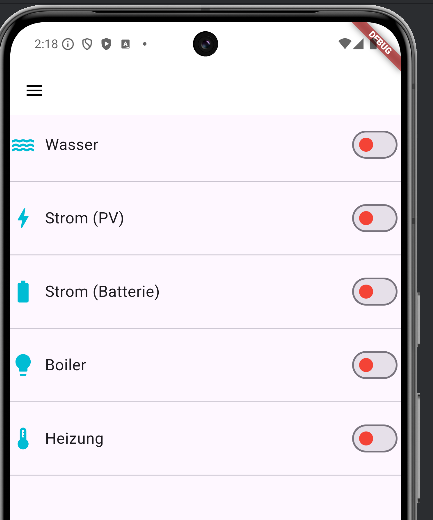
\includegraphics[height=4cm]{images/FrontEndScreenshot}
        \caption{Frontend der EnergyApp mit grundlegenden Funktionen}
    \end{figure}
    Das Menü wird über einen sogenannten \enquote{AppDrawer} realisiert, der sich oben links befindet und
    durch eine Berührung aufgerufen werden kann.
    Dieser Drawer wurde mit Hilfe von ChatGPT entwickelt und bietet Zugriff auf weitere Funktionen der Anwendung. \\
    Ein Klick auf \enquote{Wasser} hat derzeit keine Funktion, da dieser Button als Dummy-Funktion dient. \\
    Hingegen führen Klicks auf \enquote{Boiler} oder \enquote{Heizung} dazu, dass mithilfe der Funktion
    \enquote{MaterialPageRoute} eine Navigation in die nächste Ansicht erfolgt.
    Dabei wird eine neue Seite geladen, die die Graphen aufruft.
    Eine detaillierte Beschreibung folgt in einem späteren Abschnitt des Dokuments.

    \begin{lstlisting}[language=Dart]
class MainScreen extends StatelessWidget {
    // ...
      drawer: AppDrawer(database: database),
      body: Column(
        children: [
          ToggleItem(
            icon: Icons.water,
            label: "Wasser",
            onTap: () {},
          ),

    // ...

        ToggleItem(
  icon: Icons.lightbulb, // Placeholder for Boiler icon
  label: "Boiler",
  onTap: () {
    Navigator.push(
      context,
      MaterialPageRoute(builder: (context) =>
                    StockScreenV3(database: database)), // ....
    \end{lstlisting}
    Die Funktion \enquote{AppDrawer} implementiert ein seitliches Navigationsmenü, das sich von der linken Seite des
    Bildschirms aus öffnet.
    Dieses Menü nimmt etwa die Hälfte des Bildschirms ein und enthält sowohl einige Dummy-Funktionen
    als die neu implementierte Funktionen \enquote{Erweiterte Statistik}, die in einem späteren Kapitel detailliert
    beschrieben werden.
    Ein Klick außerhalb des Menüs führt zurück zum \enquote{Hauptbildschirm}

 \begin{figure}
    \centering
    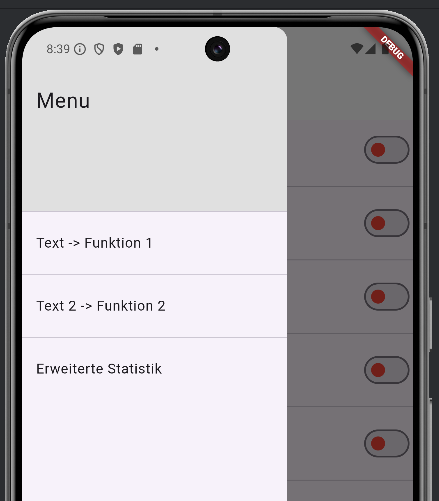
\includegraphics[height=4cm]{images/MenueScreen}
    \caption{Menüansicht, relevant ist die Funktion \enquote{Erweiterte Statistik}.}
\end{figure}

\newpage

\section*{Statistik}
    Mit dem Aufruf der \enquote{Erweiterten Statistik} werden die Methoden der Datei \enquote{Gesamtstatistik.dart}
    getriggert. \\
    Zunächst erfolgt die Initialisierung einiger Variablen, die im weiteren Verlauf mit Werten befüllt und je nach
    Bedarf wieder geleert werden. \\
    Im weiteren Verlauf des Codes gibt es zudem mehrere Aufrufe an die Datei \enquote{postgresDatabase.dart},
    in der alle Datenbankabfragen gebündelt sind. \\
    Da wir eine eigene Datenbank erstellt haben, haben wir auch mit selbst definierten Dummydaten gearbeitet,
    die für uns realistisch Klangen und daher auch potenziell im Hauptsystem verwendet werden könnten.

    \begin{lstlisting}[language=Dart]
@override
Widget build(BuildContext context) {
  return Scaffold(
      appBar: AppBar(
        title: Text("Gesamtstatistik"),
 //...
        TextButton(
  onPressed: () async {
    setState(() {
      isYearly = true;
      _loadYearlyData();
    });
// ...
    ElevatedButton(
  onPressed: () {
    setState(() {
      isYearly = false;
      _loadDailyData();
    });
  },
// ...
      ),
  if (isYearly) _buildYearlyToggleButton(),
      Expanded(
    child: isYearly ? _buildYearlyView() : _buildDailyView(),
      ),
    ],
 // ...
}
    \end{lstlisting}
    Die \enquote{build()}-Methode ist dafür zuständig, die Seite der erweiterten Statistik initial zu laden.
    Zu Beginn wird standardmäßig die Jahresstatistik durch den Aufruf von \enquote{\_buildYearlyView()} dargestellt. \\
    Zusätzlich enthält die Methode zwei Buttons, mit denen der Nutzer zwischen der jährlichen, also \enquote{\_buildYearlyView}, und täglichen, \enquote{\_buildDailyView}, Statistik wechseln kann.
    Je nach Auswahl werden die entsprechenden Bildschirme geladen und den damit verbundenen Statistikdaten.
    \\ \\ \\
    \begin{lstlisting}[language=Dart]
Future<void> _loadYearlyData() async {
    try {
        if (widget.database.connection.isClosed) {
        widget.database.connectToDatabase();
        }
        yearlyData = await widget.database.fetchYearlyStatistics();
        setState(() {});
    } catch (e) {
    print("Fehler beim Laden der Jahresdaten: $e");
    }
}
    \end{lstlisting}
    In dieser Methode wird zunächst überprüft, ob die Verbindung zur Datenbank noch aktiv ist.
    Da wir festgestellt haben, dass bei längerer Inaktivität der App die Verbindung automatisch getrennt wird. \\
    Falls die Verbindung geschlossen ist, wird sie mithilfe der bereits in der \enquote{main.dart} vorgestellten
    Methode erneut hergestellt.
    Ist die Verbindung noch aktiv, wird direkt mit dem Abruf der jährlichen Statistik fortgefahren.
    Nach dem erfolgreichen Abruf der Daten aus der Datenbank wird die Benutzeroberfläche mithilfe von
    \enquote{setState()} aktualisiert, sodass die neuen Daten unmittelbar im UI dargestellt werden.

    \begin{lstlisting}[language=Dart]
Future<List<Map<String, dynamic>>>
                    fetchYearlyStatistics() async {
  try {
    if(connection.isClosed) {
      connectWithRetry();
    }
    List<List<dynamic>> results = await connection.query('''
    SELECT
      jahr,
      COUNT(DISTINCT CASE WHEN batterie_status = 100 THEN DATE(
            jahr || '-' || monat || '-' || tag) END)
                                         AS anzahl_batterie_100,
      COUNT(DISTINCT CASE WHEN boiler_temp > 100 THEN DATE(
            jahr || '-' || monat || '-' || tag) END)
                                      AS anzahl_boiler_ueber_140
    FROM gesamtstatistik
    GROUP BY jahr
    ORDER BY jahr DESC;
    ''');

    return results.map((row) {
      return {
        'Jahr': row[0],
        'anzahl_batterie_100': row[1],
        'anzahl_boiler_ueber_140': row[2],
      };
    }).toList();
  } catch (e) {
    print('Fehler beim Abrufen der Jahresstatistik: $e');
    return [];
} }
    \end{lstlisting}
    Die Methode \enquote{fetchYearlyStatistics()} wird von \enquote{loadYearlyData()} aufgerufen und gehört zur Klasse
    \enquote{postgresDatabase}.
    Diese Trennung wurde bewusst vorgenommen, um alle Datenbankzugriffe in einer eigenen Klasse zu kapseln und
    den Code übersichtlicher zu gestalten.  \\
    Zu Beginn wird überprüft, ob eine Verbindung zur Datenbank aktiv ist.
    Falls die Verbindung geschlossen ist, wird die Methode \enquote{connectWithRetry()} aufgerufen, die eine Wiederherstellung der
    Verbindung mit Verzögerungen versucht.
    Nach erfolgreicher Verbindung wird eine SQL-Abfrage ausgeführt, deren Ergebnisse in einer dynamischen Liste
    gespeichert werden.
    Die Abfrage zählt die Anzahl der Tage pro Jahr, an denen:
    \begin{itemize}
        \item die Batterie einen Ladezustand von 100\% erreicht hat, und
        \item die Temperatur des Boilers 100 Grad überschritten hat.
    \end{itemize}
    Diese Selektion erfolgt durch die SQL-Funktion \enquote{COUNT(DISTINCT ...)}, die alle eindeutigen Tage zählt, an
    denen die jeweiligen Bedingungen erfüllt wurden.
    Diese Methode basiert auf dem Prinzip, welches wir in der Vorlesung \enquote{Datenbanken 1} gelernt haben.

    \begin{lstlisting}[language=Dart]
Widget _buildYearlyView() {
  return SingleChildScrollView(
    scrollDirection: Axis.horizontal,
    child: DataTable(
      columns: const [
        DataColumn(label: Text('Jahr')),
        DataColumn(label: Text('Batterie > 100%')),
        DataColumn(label: Text('Boiler > 100C')),
      ],
      rows: yearlyData.map((data) {
        int year = data['Jahr'];
        int daysInYear = isLeapYear(year) ? 366 : 365;
        return DataRow(cells: [
          DataCell(Text('${data['Jahr']}')),
          DataCell(Text(showPercentage
              ? '${(data['anzahl_batterie_100'] / daysInYear * 100)
              .toStringAsFixed(2)}%'
              : '${data['anzahl_batterie_100']} / $daysInYear')),
          DataCell(Text(showPercentage
              ? '${(data['anzahl_boiler_ueber_140'] / daysInYear * 100)
              .toStringAsFixed(2)}%'
              : '${data['anzahl_boiler_ueber_140']} / $daysInYear')),
        ]);
      }).toList(),
    ),
  );
}
    \end{lstlisting}

    Die Methode \enquote{\_buildYearlyView()} holt die Werte aus der zuvor aufgerufenen Methode
    \enquote{\_loadYearlyData()} und verarbeitet diese zur Anzeige in einer \enquote{DataTable}.
    Die Tabelle besteht aktuell aus 3 Spalten und gibt die Anzahl an Tagen, in der sie ihre Abfrage erreicht hat.
    Die Werte für Batterie und Boiler können entweder \textbf{als absolute Anzahl der Tage oder als prozentualer Anteil}
    der gesamten Tage im jeweiligen Jahr angezeigt werden, welche durch \enqoute{showPercentage} gesteuert werden.
    Zusätzlich wird berücksichtigt, ob das Jahr ein Schaltjahr ist, da Schaltjahre 366 Tage haben, während normale Jahre 365 Tage umfassen.
    Diese Berechnung erfolgt mit der Methode \enquote{isLeapYear(year)}. \\
    Durch die Verwendung von \enquote{SingleChildScrollView} mit \enquote{Axis.horizontal} wird sichergestellt,
    dass die Tabelle scrollbar bleibt, falls die Inhalte über den verfügbaren Platz hinausgehen.

    \begin{lstlisting}[language=Dart]
Future<void> _loadDailyData() async {
  try {
    if (widget.database.connection.isClosed) {
      await widget.database.connectToDatabase();
    }
    if (fromDate != null && toDate != null) {
      dailyData = await widget.database.fetchDailyStatistics(
        startDate: fromDate,
        endDate: toDate,
      );
    } else if (fromDate != null && toDate == null) {
      dailyData = await widget.database.fetchDailyStatistics(
        startDate: fromDate,
      );
    } else if (fromDate == null && toDate != null){
      dailyData = await widget.database.fetchDailyStatistics(
        endDate: toDate,
      );
    } else {
      dailyData = await widget.database.fetchDailyStatistics();
    }
    setState(() {});
  } catch (e) {
    print("Fehler beim Laden der Tagesdaten: $e");
  }
}
    \end{lstlisting}
    Das Laden der täglichen Statistiken funktioniert grundsätzlich ähnlich wie bei der jährlichen Version.
    Der wesentliche Unterschied besteht jedoch darin, dass hier ein zusätzlicher Datumsfilter integriert wurde.
    Dieser Filter ermöglicht es, die Daten gezielt nach bestimmten Tagen oder Zeiträumen zu durchsuchen.
    Dadurch lassen sich einerseits unnötig große Datenmengen vermeiden und andererseits einzelne Tage gezielt analysieren.
    \begin{lstlisting}[language=Dart]
Future<List<Map<String, dynamic>>>
    fetchDailyStatistics({DateTime? startDate, DateTime? endDate}) async {
  try {
    if (connection.isClosed) {
      connectWithRetry();
    }
    String query = '''
    SELECT DISTINCT ON (Jahr, Monat, Tag)
      Jahr, Monat, Tag, MAX(batterie_status)
            AS batterie_status, MAX(boiler_temp) AS boiler_temp
    FROM gesamtstatistik
  ''';
    List<String> conditions = [];
    if (startDate != null && endDate != null) {
      conditions.add('Jahr >= ${startDate.year}
                                    AND Jahr <= ${endDate.year}');
      conditions.add('Monat >= ${startDate.month}
                                    AND Monat <= ${endDate.month}');
      conditions.add('Tag >= ${startDate.day}
                                    AND Tag <= ${endDate.day}');
    } else if (startDate != null && endDate == null) {
      conditions.add('Jahr >= ${startDate.year}');
      conditions.add('Monat >= ${startDate.month}');
      conditions.add('Tag >= ${startDate.day}');
    } else if (startDate == null && endDate != null) {
      conditions.add('Jahr <= ${endDate.year}');
      conditions.add('Monat <= ${endDate.month}');
      conditions.add('Tag <= ${endDate.day}');
    }
    if (conditions.isNotEmpty) {
      for(int i = 0; i < conditions.length; i++){
        if(i == 0){
          query += '\nWHERE ' + conditions.elementAt(i);
        } else {
          query += '\nAND ' + conditions.elementAt(i);
        }
      }
    }
    query += '\nGROUP BY Jahr, Monat, Tag\n
                    ORDER BY Jahr DESC, Monat DESC, Tag DESC';
    List<List<dynamic>> results = await connection.query(query);
    return results.map((row) {
      return {
        'Jahr': row[0],
        'Monat': row[1],
        'Tag': row[2],
        'batterie_status': row[3],
        'boiler_temp': row[4],
      };
    }).toList();
  } catch (e) {
    print('Fehler beim Abrufen der Tagesstatistik: $e');
    return [];
  }
}
    \end{lstlisting}
    In dieser Methode wird die SQL-Abfrage nicht direkt als fester String definiert, sondern als
    dynamischer String aufgebaut und während der Laufzeit ergänzt.
    Dies ermöglicht eine flexible Anpassung der Abfrage je nach den angegebenen Filterparametern.
    Mit der SQL-Funktion \enquote{MAX()} werden die höchsten Werte für \enquote{batterie\_status} und
    \enquote{boiler\_temp} pro Tag abgerufen.
    Durch die Kombination mit \enquote{GROUP BY Jahr, Monat, Tag} wird sichergestellt, dass die Werte für
    jeden einzelnen Tag separat aggregiert werden. \\
    Die Sortierung erfolgt mit \enquote{ORDER BY Jahr DESC, Monat DESC, Tag DESC}, sodass die neuesten
    Daten zuerst geladen und verarbeitet werden.
    Dadurch wird eine chronologisch absteigende Darstellung gewährleistet, bei der die aktuellsten
    Messwerte oben stehen und ältere Werte weiter unten folgen. \\
    Nach der finalen Zusammenstellung wird der SQL-String an die Datenbank gesendet.
    Die zurückgegebenen Ergebnisse werden in eine dynamische Liste umgewandelt, die dann weiterverarbeitet werden kann.
    Die beiden SQL-Abfragen sind recht flexibel und können mit kleineren Anpassungen mit anderen
    Tabellenstrukturen verwendet werden.
    \begin{lstlisting}[language=Dart]
Widget _buildDailyView() {
  final int pageCount = (dailyData.length / itemsPerPage).ceil();
  return Column(
    children: [
      _buildDateFilter(),
      if (dailyData.isEmpty)
        Expanded(
          child: Center(
            child: Text('Daten werden geladen.'),
          ),
        )
      else
      Expanded(
        child: Column(
        children: [
          Expanded(
            child: SingleChildScrollView(
              scrollDirection: Axis.vertical,
              child: SingleChildScrollView(
                scrollDirection: Axis.horizontal,
                child: DataTable(
                  columns: const [
                    DataColumn(label: Text('Datum')),
                    DataColumn(label: Text('Batterie = 100%')),
                    DataColumn(label: Text('Boiler > 100C')),
                  ],
    // ...
    \end{lstlisting}
    Zunächst beginnt das Widget mit der Erstellung der und fragt ab, ob Daten überhaupt vorhanden sind, ist dies der Fall, wird ein Ladebildschirm imitiert,
    da wir sonst auf Fehler auf visuelle Fehler in der App kommen.
    Da alles Asynchron passiert wird währenddessen der Datumsfilter gebaut, welcher uns die einfache Möglichkeit erstellt,
    nach einem Datum zu sortieren.
    Im weiteren Verlauf wird die 3 Spaltenbreite Tabelle initialisiert.

    Das Widget \enquote{\_buildDailyView()} beginnt mit der Initialisierung und überprüft, ob Daten verfügbar sind.
    Falls keine Daten vorhanden sind, wird ein Ladebildschirm generiert. \\
    Dies verhindert visuelle Fehler in der App, die auftreten könnten, wenn versucht wird, nicht vorhandene Daten anzuzeigen.
    Da alle Prozesse asynchron ablaufen, wird währenddessen der Datumsfilter (\enquote{\_buildDateFilter()}) erstellt,
    um den User das Filtern nach Tag, Monat und Jahr zu ermöglichen.
    Um die Anzeige übersichtlich zu gestalten, wird in die Tabelle eine vertikalen und horizontalen
    Scroll-Funktion versehen, (\enquote{SingleChildScrollView}).
    \begin{lstlisting}[language=Dart]
      //...
child: DataTable (
    columns: const [
        DataColumn(label: Text('Datum')),
        DataColumn(label: Text('Batterie = 100\%')),
        DataColumn(label: Text('Boiler > 100C')),
    ],
  rows: dailyData
    .skip(currentPage * itemsPerPage)
    .take(itemsPerPage)
    .map((data) {
    bool batteryReached = double.parse(data['batterie_status']) == 100;
    bool boilerExceeded = (data['boiler_temp']) > 100;
    return DataRow(cells: [
      DataCell(Text('${data['Tag'].toString().padLeft(2, '0')}.
            ${data['Monat'].toString().padLeft(2, '0')}.${data['Jahr']}')),
      DataCell(Row(
        children: [
          batteryReached
            ? Icon(Icons.check, color: Colors.green) // Gruener Haken
            : Icon(Icons.close, color: Colors.red), // Rotes X
 // Pagination Steuerung
  Row(
    mainAxisAlignment: MainAxisAlignment.center,
        children: [
          IconButton(
            onPressed: currentPage > 0
            ? () {
              setState(() {
                currentPage--;
              });
            }
                : null,
            icon: Icon(Icons.arrow_back),
            ),
            Text('Seite ${currentPage + 1} von $pageCount'),
            IconButton(
            onPressed: currentPage < pageCount - 1
            ? () {
            setState(() {
                currentPage++;
            });
            }
    // ...
    }
    \end{lstlisting}
    Die Daten aus den Datenbankaufrufen werden aus DailyData entzogen und weiter verarbeitet. Sollte die Batterie an
    jenem Tag 100 Prozent erreicht haben oder der Boiler 100 Grad wird für diesen Tag ein Haken gesetzt,
    andernfalls ein rotes Kreuz. Weiters wurde mittels itemsperPage initialisiert wie viele Daten pro Seite
    angezeigt werden dürfen, um das Gerät zu entlasten und nicht tausende von Einträge zu haben.
    Initial wurde dies auf 40 Einträge pro Seite limitiert und durch die Länge der Liste und der Anzahl der Items werden
    die Anzahl der Seiten bestimmt. \\
    Weiter wurden Pfeile implementiert, die sog. IconButtons, welche durch die Seiten hin durch navigieren können.
    Die Daten aus den Datenbankabfragen werden aus \enquote{dailyData} entnommen und zur Anzeige weiterverarbeitet.
    Falls die Batterie an einem bestimmten Tag eine Ladung von \enquote{100\%} erreicht hat oder der Boiler eine
    Temperatur von über 100 Grad überschritten hat, wird für diesen Tag ein grüner Haken angezeigt.
    Andernfalls erscheint ein rotes Kreuz.

\newpage

\section*{Graphen}

In diesem Teil wird genauer erklärt wie der Teil funktioniert, der für die graphische Darstellung verantwortlich ist. Dabei wird zuerst geklärt wie auf die Daten in der Datenbank zugegriffen wird und dann wie diese Daten verarbeitet werden.

\subsection*{postgresDatabase}

In dieser Datei befinden sich die Methoden die den 
Zugriff und Datenaustausch mit der Datenbank ermöglichen. Von Interesse sind für uns 7 verschiedene Methoden. 

\begin{lstlisting}[language=Dart]

fetchLast24HoursData(String tableName)
fetchLast5DaysData(String tableName)
fetchMonthData(String tableName)
fetch6MonthData(String tableName)
fetchYearlyData(String tableName)
fetchCurrentYearlyData(String tableName)
fetchYearlyMaxData(String tableName)

\end{lstlisting}

Diese ermöglichen uns wie schon im Namen erklärt Zugriff auf Daten in bestimmten Abständen(1 Tag, 5 Tage, 1 Monat, 6 Monate, 1 Jahr, jetzige Jahr und alle Jahre bis jetzt.) Diese Methoden sind dabei immer nach dem selben Prinzip aufgebaut und unterscheiden sich nur in der SQL anfrage die sie ausführen, die für die Einholung der Daten zuständig ist.

Wir werden dies nun am Beispiel von fetchYearlyData durchgehen.
Zuerst wird eine Verbindung zur DB aufgebaut.

\begin{lstlisting}[language=Dart]

try {
      if (connection.isClosed) {
        connectWithRetry();
      }

\end{lstlisting}

Danach wird die Zeitspanne der benötigten Daten ermittelt die später für die SQL Anfrage benötigt werden.

\begin{lstlisting}[language=Dart]

// Calculate the date range for the past year
      DateTime now = DateTime.now();
      DateTime endDate = now;
      DateTime startDate = now.subtract(Duration(days: 365));

      // Extract year and month for the start and end dates
      int startYear = startDate.year;
      int startMonth = startDate.month;

      int endYear = endDate.year;
      int endMonth = endDate.month;

\end{lstlisting}

Die vorher ermittelten Daten basierend auf der aktuellen Zeit werden daraufhin in eine SQL Anfrage eingefügt.

\begin{lstlisting}[language=Dart]

// Build the query to calculate monthly mean temperature for the past year
      String query = """
    SELECT year, month, AVG(temperature) AS mean_temperature
    FROM $tableName
    WHERE 
      (year > $startYear OR (year = $startYear AND month >= $startMonth))
      AND
      (year < $endYear OR (year = $endYear AND month <= $endMonth))
    GROUP BY year, month
    ORDER BY year, month;
    """;

\end{lstlisting}

Die von der DB erhalten Daten nach Ausführen der Anfrage werden in eine Liste gespeichert. Die Daten werden dabei mit Feldern verknüpft um den späteren Zugriff zu erleichtert

\begin{lstlisting}[language=Dart]

// Execute the query
      List<List<dynamic>> results = await connection.query(query);

      // Map the results to the expected structure
      return results.map((row) {
        return {
          'Year': row[0],
          'Month': row[1],
          'Temperature': row[2],
        };
      }).toList();

\end{lstlisting}

Der einzige weitere Unterschied den diese Methoden haben ist von welchen Zeitabständen her die Daten eingeholt werden. Den während für die tägliche Grafik die Daten in 15 Minuten von Interesse wären, ist für das grafische Darstellung des jährlichen Graphen der Monatlich Durchschnitt wichtiger und auch leichter grafisch darzustellen als Daten in 15 Minuten Abständen. Die genaueren Gründe dafür werden im nächsten Teil erläutert.

Die Zeitabstände/Durchschnitt der Zeitabstände der jeweiligen Methoden lauten:
\begin{itemize}[noitemsep, topsep=0pt]
    \item 1 Tag: 15 Minuten
    \item 5 Tage: 1 Stunde
    \item 1 Monat: Durchschnitt pro Tag
    \item 6 Monat: Durchschnitt pro Monat
    \item 1 Jahr: Durchschnitt pro Monat
    \item jetziges Jahr: Durchschnitt pro Monat
    \item alles bis jetzt: Durchschnitt pro Monat
\end{itemize}

\subsection*{stock screen v2}

In dieser Datei befinden sich die Methoden und Code, welche die Daten aus der DB verwerten und diese dann grafisch darzustellen.

Am Anfang der Datei werden 2 Arten von Listen erstellt. Einmal jene die Daten aus der DB speichern sollen

\begin{lstlisting}[language=Dart]

List<Map<String, dynamic>> yearData = [];

\end{lstlisting}

und zweitens Listen die FlSpots speichern sollen.

\begin{lstlisting}[language=Dart]

List<FlSpot> chart1Data1Year = [];

\end{lstlisting}

Diese FlSpots sind umgewandelte Datensätze aus der Datenbank die das grafische darstellen ermöglichen.

Diese Listen werden gleich beim Start der App vorbereitet damit sie sofort zugreifbar sind. Dies erfolgt durch die Methode loadData(). Diese verbindet sich zuerst mit der DB und greift danach auf die nötigen Daten zu.

\begin{lstlisting}[language=Dart]

dayData = await widget.database.fetchLast24HoursData('boiler');
day5Data = await widget.database.fetchLast5DaysData('boiler');
monthData = await widget.database.fetchMonthData('boiler');
month6Data = await widget.database.fetch6MonthData('boiler');
yearCurrentData = await widget.database.fetchCurrentYearlyData('boiler');
yearData = await widget.database.fetchYearlyData('boiler');
yearAllData = await widget.database.fetchYearlyMaxData('boiler');

dayDataB2 = await widget.database.fetchLast24HoursData('boiler2');
day5DataB2 = await widget.database.fetchLast5DaysData('boiler2');
monthDataB2 = await widget.database.fetchMonthData('boiler2');
month6DataB2 = await widget.database.fetch6MonthData('boiler2');
yearCurrentDataB2 = await widget.database.fetchCurrentYearlyData('boiler2');
yearDataB2 = await widget.database.fetchYearlyData('boiler2');
yearAllDataB2 = await widget.database.fetchYearlyMaxData('boiler2');

\end{lstlisting}

Nachdem die Daten geladen wurden wird die Methode getFLSpotDataReady() aufgerufen. Diese wandelt wie vorher besprochen die Daten zu FlSpots mithilfe der Methode convertToFlSpots(List<Map<String, dynamic>> data).

\begin{lstlisting}[language=Dart]

return List<FlSpot>.generate(data.length, (index) {
      final temperature = data[index]['Temperature'];
      if (temperature is! double && temperature is! int) {
        throw ArgumentError(
          'Invalid temperature value at index $index: $temperature.
          It must be a number.',
        );
      }
      return FlSpot(index.toDouble(), temperature.toDouble());
    });
    
\end{lstlisting}

Hierbei ist nur die zeitliche Abfolge und Temperatur der Daten von Interesse. Durch die SQL Abfrage werden die Datensätze schon zeitlich richtig sortiert, wobei diese Reihenfolge als unsere x-Werte für die Punkte in unserem Koordinatensystem hergenommen werden. Die Temperatur wiederum dient als unser y-Wert für die Punkte.

Der nächste Schritt ist das erstellen unserer graphischen Oberfläche. Dabei gibt es 7 auswählbare Tabs, wobei die tägliche Grafik als Standard ausgewählt ist.
Dazu gibt es noch eine Kurzbeschreibung, die je nach angewählten Tab ausgewählt wird.

\begin{lstlisting}[language=Dart]

tabs: [Tab(text: "1T"), Tab(text: "5T"), Tab(text: "1M"),
Tab(text: "6M"), Tab(text: "YTD"), Tab(text: "1J"),
Tab(text: "MAX")]

String getTimeDescription() {
    switch (selectedTab) {
      case 0: return "1 Nov, 15:40:40";
      case 1: return "Last 5 Days";
      case 2: return "Last 1 Month";
      case 3: return "Last 6 Months";
      case 4: return "Year to Date";
      case 5: return "Last 1 Year";
      case 6: return "Last 6 Years";
      default: return "";
    }
}
    
\end{lstlisting}

Danach wird die Grafik erstellt. Da große Datenmengen geladen werden, kann es zu leichten Zeitverzögerungen kommen. Diese verursachten während unserer Testphase mehrfach Fehler. Um diesen Fehler zu lösen überbrücken wir ihn mit einem Ladebildschirm, der verhindern soll das auf leere Daten zugegriffen wird.

\begin{lstlisting}[language=Dart]

if (getChartDataFromDB().isEmpty)
              Expanded(
                child: Center(
                  child: Text('Daten werden geladen.'),
                ),
              )
    
\end{lstlisting}

Als nächstes kommt die Erstellung der Grafik. Dafür müssen wir die Minimums und Maximums für die x- und y-Werte ermitteln. Für den x-Wert ist es einfach- Min ist  0 und der letzte Index in der Liste ist das Max.

\begin{lstlisting}[language=Dart]

minX: 0,
maxX: getChartDataFromDB().last.x
    
\end{lstlisting}

Für den y-Wert wird es ein wenig komplexer. Gelöst wird das ganze durch ein Vergleich der Min und Max y-Werte der FlPoints der verschiedenen Datensätze(Bei 2 oder mehr Graphen) bei den Methode getMinY() und getMaxY(). Ansonsten kann einfach das Min und Max eines Datensatzes(1 Graph) hergenommen werden ohne einen Vergleich. Der Intervall der y-Achse wird dabei auf 5 Beschriftungen begrenzt mithilfe des unterem Codeteils.

\begin{lstlisting}[language=Dart]

interval: (getMaxY() - getMinY()) / 4, // Ensure 5 labels (0 to 4 intervals)
    
\end{lstlisting}

Ein weiterer wichtiger Punkt ist die dynamische Beschriftung der x-Achse je nach Zeitspanne oder verschiedenen Zeitpunkten. Gelöst wird dies durch die Setzung eines dynamischen Intervalls mithilfe der getInterval und getXAxisLabels Methode.

\newpage

\begin{lstlisting}[language=Dart]

interval: getInterval(),
getTitlesWidget: (value, _) => getXAxisLabels(value)

\end{lstlisting}

Die Methode getInterval() funktioniert folgendermaßen: Wir erhalten eine unterschiedliche Anzahl an FlPoints, die alle eingezeichnet werden, je nach Tab in dem wir uns gerade befinden. Einige Punkte an der x-Achse wollen wir aber angezeigt bekommen, in unserem Fall die Zeitabstände. Wenn wir beispielsweise 96 FlPoints bekommen, weil wir für 24 Stunden pro Stunde 4 Datenpunkte erhalten wegen dem 15 Minuten Unterschied, dann müssen wir einen Intervall wählen der auf diese Anzahl zugeschnitten ist. In unserem Fall wollten wir einen Zeitabstand von 3 Stunden anzeigen. $96 \div 12 = 8$ Beschriftungen. $8 \times 3 = 24$ Stunden Darstellung. Das selbe Prinzip trifft auch auf die anderen Intervalle zu.

\begin{lstlisting}[language=Dart]

double getInterval() {
    //regulates how many intervals are set through the x axis
    switch (selectedTab) {
      //96Inputs-15min interval
      case 0: return 12;
      //120Inputs-1h interval
      case 1: return 24;
      //30Inputs-7d interval
      case 2: return 7;
      //6Inputs-1m Interval
      case 3: return 1;
      //1-12Inputs-1m Interval
      case 4: return 2;
      //12Inputs-1y Interval
      case 5: return 2;
      //1-maxInputs-1m Interval
      case 6: return 12;
      default: return 1;
\end{lstlisting}

Dadurch bekommen wir aber nicht die passenden x-Achsen Beschriftungen sondern nur die richtigen Abstände. Um die passenden Beschriftungen zu bekommen brauchen wir getXAxisLabels(double value). Diese berechnet anhand der Anzahl der FlPoints die Zeitspanne, welche dargestellt wird.

\begin{lstlisting}[language=Dart]

DateTime now = DateTime.now();
    switch (selectedTab) {
      case 0: return Text(DateFormat('HH:mm').
      format(now.add(Duration(minutes: 15 * value.toInt()))),
      style: TextStyle(color: Colors.grey, fontSize: 10));
\end{lstlisting}

Gehen wir dies anhand des täglichen Tabs durch. Zuerst wird die aktuelle Zeit berechnet. Danach wird mit Dateformat, die Form der Beschriftung festgelegt. In diesem Fall wäre das \enquote{Stunden : Minuten}. Nun kommen wir zur eigentlichen Berechnung. Mit now.add wird festgelegt das zu jetzigen Zeit etwas hinzuaddiert werden soll. Mit \enquote{minutes: } wird die Einheit fixiert. Mit \enquote{15 $\times$ value.toInt()} wird nun für jeden FlPoint der durchgegangen wird 15 Minuten zur jetzigen Zeit hinzuaddiert. Somit erreicht man einen 24 Stunden Zyklus mit 96 FlPoints. Normalerweise wird bei den anderen Zeitspannen \enquote{now.substract} verwendet um vergangene Zeit darzustellen, aber bei der täglichen Zeitspanne macht es keinen Unterschied.

Zu guter Letzt wird mit

\begin{lstlisting}[language=Dart]

LineChartBarData(
    spots: getChartDataFromDBB2(),
    isCurved: true,
    color: Colors.green,
    barWidth: 2,
    belowBarData: BarAreaData(show: false, 
            color: Colors.green.withOpacity(0.2)),
    dotData: FlDotData(show: false), // Disable the dots
                        
\end{lstlisting}

der eigentliche Graph eingezeichnet. Zusätzlich zu sehen sind einige Optionen wie man diesen Graph anpassen könnte.

\subsection*{stock screen v3}

Stockscreen v2 ist von Stockscreen v3 nicht wirklich unterscheidbar. Das einzige was sie wirklich unterscheidet ist, dass bei der v2 zwei Graphen eingezeichnet werden und bei v3 nur einer. Code technisch unterscheiden sie sich in sehr wenigen Dingen. Einerseits werden in v3 keine zwei verschiedenen Tabellen mit Daten benötigt um mehrere Graphen einzuzeichnen weswegen es nur halb so viele Listen gibt und auch bei den lade Methoden nur eine Tabelle geladen wird. Wie schon erwähnt werden die y-Achsen Werte unterschiedlich berechnet und es wird auch kein zweites LineChartBarData() benötigt um den zweiten Graphen zu erstellen. Im Grunde basieren sie aber auf dem selben Design und funktionieren gleich.

\end{document}
